
\def \Subject {گزارش پیاده سازی مدل }
\def \Course {درس یادگیری ماشین}
\def \Author {کسرا سینایی، امیرحسین افخمی}
\def \Report {گزارش نهایی}
\def \StudentNumber {۸۱۰۶۹۶۲۵۴، 810696206}

\begin{center}
\vspace{.4cm}
{\bf {\huge \Subject}}\\
{\bf \Large \Course}
\vspace{.2cm}
\end{center}
{\bf \Author }  \\
{\bf شماره دانشجویی:\ \StudentNumber}
\hspace{\fill} 
{\Large \Report} \\
\hrule
\vspace{0.8cm}

\clearpage

%\huge{\Subject}\\[1.5 cm]
%\chapterauthor{\Author~ : \StudentNumber}

\section{فیچر اکسترکشن}
برای رسیدن به یک مدل مناسب برای طبقه بندی و همچنین خوشه بندی، مهم ترین عامل، داشتن فیچر مناسب است.
برای استخراج فیچرهای مناسب از آهنگ‌های موجود سعی شد تا تمامی فیچرهای اصلی ممکن استخراج شود.
در مجموع 97 فیچر از آهنگ‌های موجود در دیتاست استخراج شد که در ادامه آورده شده‌اند.
لازم به ذکر است که به طور کلی دو رویکرد برای استخراج ویژگی از داده‌های صوتی وجود دارد که یکی از آن‌ها مطابق رویکردی است که در این پروژه اتخاذ شده است ودیگری 
تبدیل داده‌های صوتی به صورت فریم‌های تصویری و استفاده از این تصاویر برای تسک‌های یادگیری ماشین است.
از آن جایی که استفاده از شبکه‌های کانولوشنی در این پروژه مجاز نیست، در این جا از این روش استفاده نشد.

در فیچرهای زیر، مقادیر واریانس و میانگین به عنوان فیچر برای هر یک از آهنگ‌ها در نظر گرفته شد.

\begin{description}

    \item[$\bullet$] \lr{Chroma STFT}
    \item[$\bullet$] \lr{Spectral Centroid} 
    \item[$\bullet$] \lr{Spectral Rolloff}
    \item[$\bullet$] \lr{Spectral Bandwidth}
    \item[$\bullet$] \lr{Zero Crossing Rate}
    \item[$\bullet$] \lr{RMS Value for Each Frame}
    \item[$\bullet$] \lr{Roll-Off Frequency}
    \item[$\bullet$] \lr{Tempo}
    \item[$\bullet$] \lr{Pulse}  
    \item[$\bullet$] \lr{Harmony}
    \item[$\bullet$] \lr{:Mel-Frequency Cepstral Coefficients}
    در این فیچر میانگین و واریانس 20 \lr{MFCC} اول به عنوان فیچر در نظر گرفته شدند.
    \item[$\bullet$] \lr{:Mel-Scaled Spectrogram} 
    در این جا نیز همچون \lr{MFCC}، میانگین و واریانس 20 فیچر اول به عنوان فیچر در نظر گرفته شدند.

\end{description}

در نهایت برای هر یک از آهنگ‌ها به طور جداگانه فیچرهای فوق استخراج شدند و در یک فایل CSV ذخیره شدند.
در پایان باید به این نکته توجه داشت که تمامی فیچرهای اکسترکت شده مناسب نیستند و به اصطلاح فیچر خوبی برای تسک کلسیفیکیشن به حساب نمیایند، چرا که 
\lr{ِDiscriminability} لازم را ایجاد نمی‌کنند. برای این موضوع در قسمت‌های بعدی، تمهیداتی همچون فیچر سلکشن و فیچر ریداکشن اندیشیده شده است.

\section{پیش پردازش}
به دلیل طولانی شدن استخراج ویژگی‌ها از فایل خام داده‌ها، هر کدام از ژانرها با تابع \lr{read folder} از پوشه‌های جداگانه باز شدند و فیچرهای به دست آمده از آن‌ها در یک فایل \lr{csv} جدا ذخیره شدند. (یک بار که از تابع \lr{read songs} استفاده شد گوگل کولب دستور رانیمه کاره اجرا کرد.) بنابراین اولین مرحله از پیش پردازش داده ادغام سطرهای این فایل‌ها در یک دیتافریم است. برای راحتی کار با داده‌ها و خواندن فایل‌های اکسل از کتابخانه \lr{pandas} کمک گرفته شده است. قبل از تقسیم مجموعه آموزش و تست، جداگانه هر یک از گروه‌ها را تقسیم می‌کنیم و سپس همه آن‌ها را در آرایه‌های \lr{numpy} می‌ریزیم. به این ترتیب هم در مجموعه‌ی تست و هم در مجموعه‌ی آموزش داده‌ها بالانس خواهند بود.
\\
یکی از مسائل مهم در کار با داده‌ها نرمال بودن یا استاندارد بودن ابعاد مختلف هر یک از سمپل‌ها می‌باشد. در این پروژه اده‌های زیادی از سیگنال به دست آمده از هر آهنگ استخراج شده است و هر کدام بیان‌گر ویژگی خاصی هستند. اسکیل و بازه تغییر آن‌ها نیز متفاوت می‌باشد. برای بهبود عملکر الگوریتم‌های خوشه بندی و یا طبقه بندی قبل از انجام هر کدام از این الگوریتم‌ها تمامی سمپل‌های مجموعه آموزش و تست استاندارد شده‌اند. برای این کار نیز از انتقال \lr{standard scalar} کتابخانه \lr{sci-kit learn} استفاده شده است.
\\
برای احتیاط هر دو آرایه استانداد شده و استاندارد نشده را نگه می‌داریم اما برای آموزش و تست از از داده‌های استاندارد استفاده خواهیم کرد.




\subsection{\lr{Feature Selection}}
برای پیدا کردن بهترین فیچرهای موجود برای رسیدن به بیشترین میزان دقت طبقه بند، در این جا از تکنیک \lr{Sequential Forward Selection} استفاده شد.
برای بهینه تر کردن انتخاب فیچرها، از \lr{Floating} نیز استفاده شد.
معیار انتخاب ویژگی‌عا در فرایند فیچر سلکشن، میزان دقت طبقه بند \lr{SVM} با کرنل \lr{Linear} در نظر گرفته شد. 
به این صورت 40 فیچر اول انتخاب شدند، همچنین برای انتخاب این فیچرها از 5 \lr{Cross Validation} نیز استفاده شد.
در ادامه نمودار مربوط به دقت مدل به ازای فیچر انتخابی آورده شده است.

\begin{figure}[h!]
    \centering
    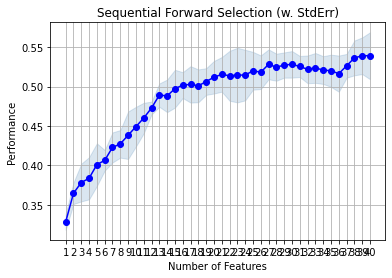
\includegraphics[width=0.75\linewidth]{images/feature_selection.png}
    \caption{انتخاب فیچرها با استفاده از \lr{SFS}}
    \label{fig:feature_selection}
\end{figure}


\section{طبقه بندی}

برای طبقه بندی از 3 الگوریتم مختلف استفاده شد. الگوریتم‌های مورد استفاده شامل \lr{SVM}، \lr{KNN} و \lr{MLP} بودند.
نتایج حاصل برای هر یک از 3 الگوریتم طبقه بند در ادامه آورده شده است.
\subsection{\lr{:SVM}}
الگوریتم \lr{soft-SVM} با استفاده از کرنل‌های مختلف پیاده سازی شد. بهترین دقت حاصل 
با در نظر گفتن کرنل \lr{Linear} و مقدار ترم \lr{Regularization} 5 بود که برابر با 55 درصد شد.
\lr{Confusion Matrix} مربوط به این طبقه بند در ادامه آورده شده است.

\begin{figure}[h!]
	\centering
	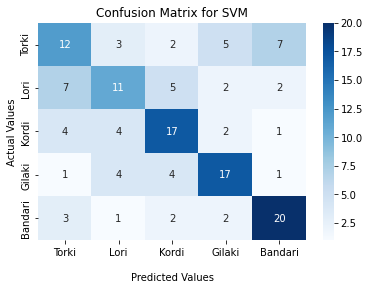
\includegraphics[width=0.75\linewidth]{images/svm_confusion_matrix.png}
	\caption{ماتریس کانفوژن برای الگوریتم \lr{SVM}}
	\label{fig:svm_confusion_matrix}
\end{figure}

میزان دقت، \lr{Precision}، \lr{Recall} و \lr{F1-score} برای این طبقه بند نیز در ادامه آورده شده است.

\begin{figure}[h!]
	\centering
	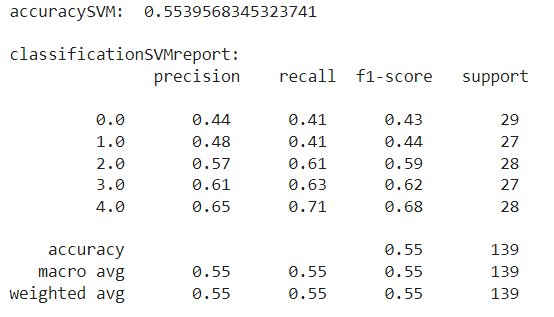
\includegraphics[width=0.9\linewidth]{images/svm_scores.PNG}
	\caption{میزان دقت، \lr{Precision}، \lr{Recall} و \lr{F1-score} برای الگوریتم \lr{SVM}}
	\label{fig:svm_scores}
\end{figure}

نتایج حاصل به دست آمده با استفاده از کرنل \lr{RBF} برای الگوریتم \lr{SVM} نیز در ادامه آورده شده است.

\newpage

\begin{figure}[h!]
	\centering
	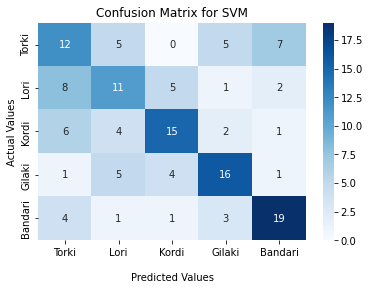
\includegraphics[width=0.75\linewidth]{images/svm_rbf_confusion_matrix.png}
	\caption{ماتریس کانفوژن به دست آمده با استفاده از کرنل \lr{RBF} برای الگوریتم \lr{SVM}}
	\label{fig:svm_rbf_confusion_matrix}
\end{figure}

\begin{figure}[h!]
	\centering
	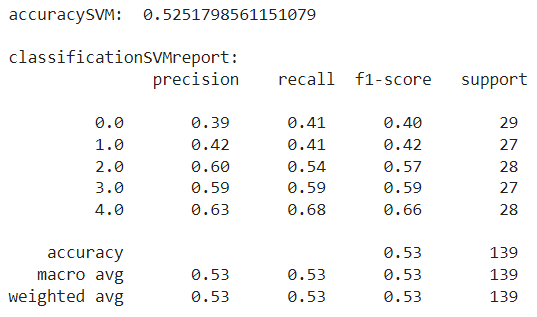
\includegraphics[width=0.9\linewidth]{images/svm_rbf_scores.PNG}
	\caption{نتایج حاصل به دست آمده با استفاده از کرنل \lr{RBF} برای الگوریتم \lr{SVM}}
	\label{fig:svm_rbf_scores}
\end{figure}

\newpage

\subsection{\lr{:KNN}}
در این الگوریتم، بیشترین میزان دقت با استفاده از در نظر گرفتن نزدیک ترین همسایه بیشترین میزان دقت بدست آمد که برابر با 51 درصد شد. 
متریک در نظر گرفته شده برای الگوریتم نزدیک ترین همسایه، فاصله اقلیدسی در نظر گرفته شد.
نتایج حاصل از طبقه بند نزدیک ترین همسایه در ادامه آورده شده است.

\begin{figure}[h!]
	\centering
	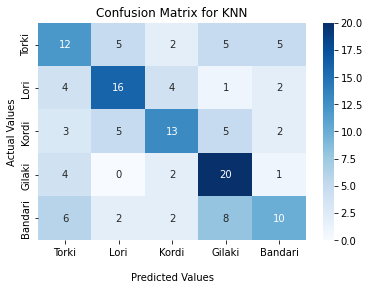
\includegraphics[width=0.75\linewidth]{images/knn_confusion_matrix.png}
	\caption{ماتریس کانفوژن برای الگوریتم \lr{KNN}}
	\label{fig:knn_confusion_matrix}
\end{figure}

\newpage

\begin{figure}[h!]
	\centering
	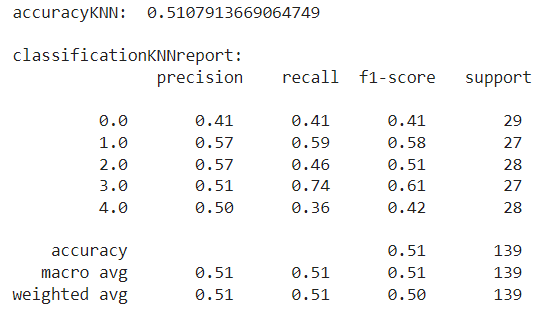
\includegraphics[width=0.9\linewidth]{images/knn_scores.PNG}
	\caption{نتایج حاصل به دست آمده برای الگوریتم \lr{KNN}}
	\label{fig:knn_scores}
\end{figure}


\subsection{\lr{:MLP}}
ساختار شبکه در نظر گرفته شده برای این الگوریتم، یک ساختار سه لایه با 128، 64 و 32 نورون در لایه پنهان است. همچنین تابع فعالساز 
\lr{ReLu} برای نورون‌های شبکه طراحی شده در نظر گرفته شد.
بین تمام لایه‌های پنهان نیز لایه دراپ اوت جهت جلوگیری از اورفیت مدل قرار داده شد. مدل در 1000 ایپاک و در بچ‌های 64 تایی آموزش داده شد.
نتایج حاصل در ادامه آورده شده است.

\begin{figure}[h!]
	\centering
	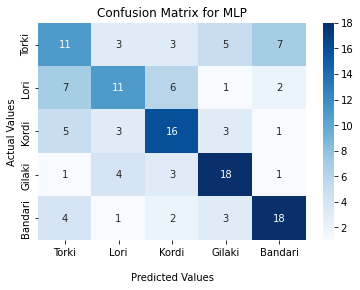
\includegraphics[width=0.75\linewidth]{images/mlp_confusion_matrix.png}
	\caption{ماتریس کانفوژن برای الگوریتم \lr{MLP}}
	\label{fig:mlp_confusion_matrix}
\end{figure}
\newpage
\begin{figure}[h!]
	\centering
	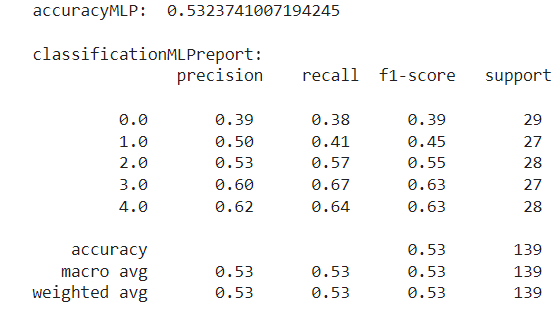
\includegraphics[width=0.9\linewidth]{images/mlp_scores.PNG}
	\caption{نتایج حاصل به دست آمده برای الگوریتم \lr{MLP}}
	\label{fig:mlp_scores}
\end{figure}



میتوان دید که بیشترین دقت به دست آمده نزدیک 55 درصد بود که دقت بسیار پایینی است. علت آن را می‌توان در فیچرهای کاهش یافته و به نمایش در آمده
در \lr{PCA} و \lr{LDA} دید. همان طور که مشخص است، فیچرها از \lr{ِDiscriminability} چندانی برخوردار نیستند
و کم بودن دیتا نیز عاملی افزاینده بر این مشکل است.

\section{خوشه بندی}
برای ایجاد یکپارچگی بین الگوریتم‌های خوشه بندی همه آن‌ها را مانند قسمت طبقه بندی به صورت متدهای یک کلاس پیاده سازی کردیم تا فرآیند آزمایش و ارزیابی آن‌ها ساده تر شود.
\\
توابع پیاده سازی شده در این کلاس هر سه نوع الگوریتم معرفی شده در درس را اجرا می‌کنند. الگوریتم \lr{K-Means} به همراه الگوریتم‌های\lr{heirarchial} و \lr{density base} در این کلاس موجود می‌باشند.
\\
برای ارزیابی الگوریتم‌ها با توجه به اینکه لیبل واقعی و درست آهنگ‌ها را می‌دانیم می‌توانیم از \lr{Purity Measure} که در کلاس درس معرفی شده است استفاده کنیم. علاوه بر این معیار یکی دیگر از معیارهای پر کاربرد برای الگوریتم‌های کلاسترینگ، \lr{Silhouette Scores} است. این معیار در بازه ۱ و ۱- قرار دارد. هر چه به ۱ نزدیک تر باشد به این معنا است که خوشهذهای به دست آمده از یکدیگر بیشتر فاصله داشته و بهتر جدا شده‌اند. در مقابل هر چه این معیار به ۱- نزدیک تر باشد به این معنی است که خوشه‌ها به یکدیگر نزدیک تر بوده و کیفیت خوشه بندی در این مسئله کمتر می‌باشد.
\\
پس از اجرای هر الگوریتم می‌توان با استفاده از متد \lr{visualize} هم معیارهای خوشه بندی ذکر شده را ملاحظه کرد و هم تصویر سه بعدی کاهش بعد یافته با استفاده از \lr{LDA} خوشه‌های به دست آمده را ترسیم کرد. توابع مورد نیاز برای محاسبه معیارهای نام برده شده جهت ارزیابی الگوریتم کلاسترینگ در کتابخانه \lr{sci-kit} به نام‌های \lr{silhouette score} و \lr{homogeniety score} موجود می‌باشند.
\\
با توجه به نمایش داده‌ها در ابعاد پایین تر می‌توان نتیجه گرفت که الگوریتم‌های خوشه بندی در این مسئله عملکرد خوبی نداشته باشند، زیرا داده‌ها کاملا در یکدیگر فرو رفته اند و در ناحیه میانی از فضا چگالی بسیار بالایی از داده‌های مربوط به گروه‌های مختلف را شاهد هستیم.

\subsection{\lr{K-Means}}
این الگوریتم بهترین نتیجه را در بین سایر الگوریتم‌های خوشه بندی در پی داشت. از کتابخانه \lr{scikit} مجددا در این قسمت استفاده شده است. همچنین برای بهبود عملکرد این الگوریتم لازم است داده‌ها حتما در فضایی کاهش بعد داده شده در الگوریتم استفاده شوند. نتایج این الگوریتم در شکل \ref{fig:kmeans} نشان داده شده است.

\begin{figure}[h!]
    \centering
    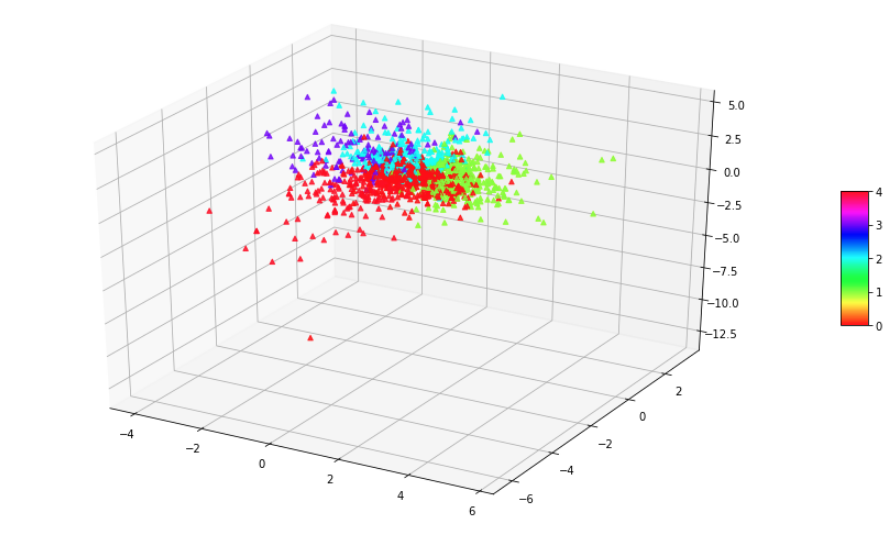
\includegraphics[width=0.65\linewidth]{images/kmeans1.png}
    \caption{نتیجه خوشه بندی با روش \lr{K Means}}
    \label{fig:kmeans}
\end{figure}

\subsection{\lr{Heirarchial Methods}}
در این قسمت با استفاده از روش \lr{bottom-up} و معیار \lr{ward} برای تعیین فاصله خوشه‌ها الگوریتم خوشه بندی \lr{Heirarchial} را اجرا می‌کنیم. برای فاصله نقاط، فاصله اقلیدسی در نظر گرفته شده است اما امکان استفاده از سایر فاصله‌های موجود در کتابخانه \lr{scipy}  و \lr{sklearn} استفاده کرد. برای پیاده سازی الگوریتم اصلی می‌توان از تابع \lr{AgglomerativeClustering} استفاه کرد و همچنین برای رسم \lr{dendogram} از تابع \lr{shc} کتابخانه \lr{scipy} کمک گرفت.

خوشه‌های به دست آمده با این روش و همچنین دندوگرام الگوریتم در شکل \ref{fig:ward} نشان داده شده‌اند.
\begin{figure}[h]
    \centering
    \subfigure[خوشه‌های به دست آمده]{
    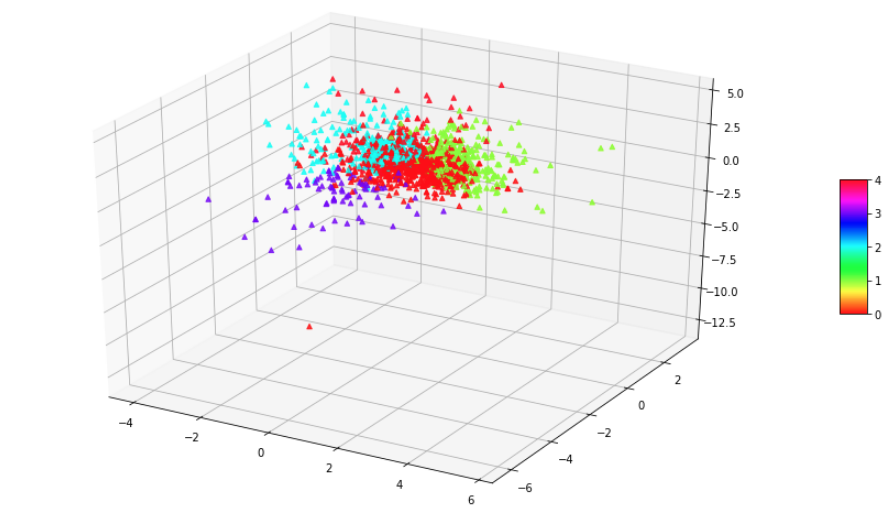
\includegraphics[width=.45\textwidth]{images/ward1.png}
    }
    \subfigure[\lr{Dendogram}]{
    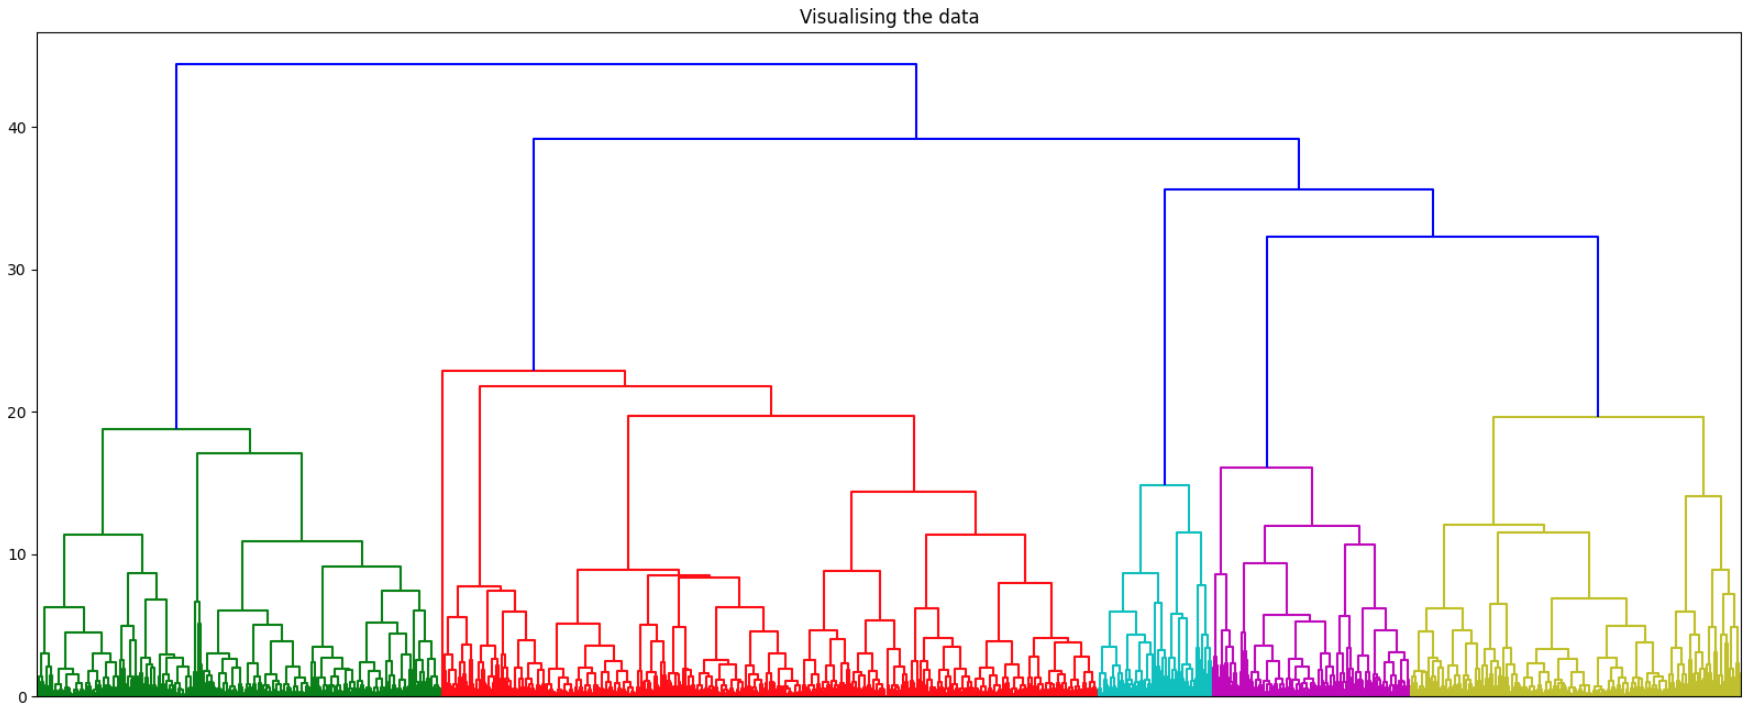
\includegraphics[width=.45\textwidth]{images/ward_dendo1.png}
    }
    \caption{نتیجه خوشه بندی با معیار \lr{ward}}
    \label{fig:ward}
\end{figure}

\subsection{\lr{DBSCAN}}
به دلیل چگالی بالا و تفکیک پذیری کم داده‌ها این الگوریتم نتایج جالبی  به همراه نداشته و نتوانسته است داده‌ها را به حداقل تعداد کلاس مورد نظر (۵) تقسیم بندی کند و تنها تعداد محدودی داده به عنوان \lr{outlier} شناسایی شدند.
\\
نتایج بد این طبقه بندی نیز در شکل \ref{fig:dbscan} نشان داده شده‌اند.

\begin{figure}[h!]
    \centering
    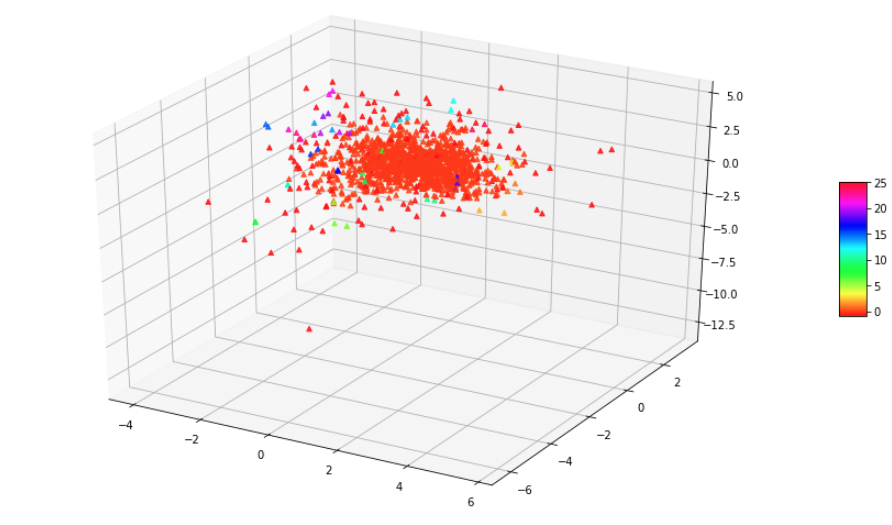
\includegraphics[width=0.65\linewidth]{images/dbscan1.png}
    \caption{نتیجه خوشه بندی با روش \lr{DBSCAN}}
    \label{fig:dbscan}
\end{figure}


در جدول زیر بین تمامی روش‌های خوشه بندی پیاده سازی شده مقایسه‌ای صورت گرفته است که بر اساس معیارهای \lr{purity} و \lr{silhouette score} می‌باشند. همانطور که مشاهده می‌شود به هیچ وجه نتایج قابل قبولی به دست نامده است.

\begin{table}[]
	\begin{tabular}{|c|c|c|c|c|c|}
	\hline
	\lr{DBSCAN} & \begin{tabular}[c]{@{}c@{}}\lr{Hierarchical}\\  (\lr{Ward})\end{tabular} & \begin{tabular}[c]{@{}c@{}}\lr{Hierarchical}\\  (\lr{Average})\end{tabular} & \begin{tabular}[c]{@{}c@{}}\lr{Hierarchical} \\ (\lr{Complete})\end{tabular} & \lr{K-Means} & \lr{Measure}    \\ \hline
	\lr{-0.164} & \lr{0.166}                                                          & \lr{0.520}                                                             & \lr{0.110}                                                              & \lr{0.204}   & \lr{Silhouette} \\ \hline
	\lr{0.106}  & \lr{0.163}                                                          & \lr{0.167}                                                             & \lr{0.109}                                                              & \lr{0.194}   & \lr{Purity}     \\ \hline
	\end{tabular}
	\end{table}

\section{\lr{Data Augmentation}}
برای حل مشکل کمبود داده، بر روی داده‌ها دیتا آگمنتیشن انجام شد، به این صورت که هر آهنگ به 5 بخش تقسیم شد و فیچرهای مورد نظر 
به صورت جداگانه از هر یک از این بخش‌ها استخراج شدند. با این کار عملا داده‌ها 5 برابر شدند. همان طور که میدانیم، برخلاف تعداد فیچر،
تعداد داده هر چقدر بیشتر باشد، کارایی مدل ما بهتر است.
این تاثیر را می‌توان در مدل‌های پیاده سازی شده در ادامه دید.

\subsection{\lr{: classification}}
نتایج حاصل از طبقه بندی با استفاده از داده‌های اضافه شده برای هر یک از الگوریتم‌ها در ادامه آورده شده است.

\subsubsection{\lr{: SVM}}
با در نظر گرفتن ترم \lr{Regularization} = 15 و 
کرنل \lr{rbf} در الگوریتم \lr{soft-SVM}
نتایج زیر حاصل گشت.



\begin{figure}[h!]
	\centering
	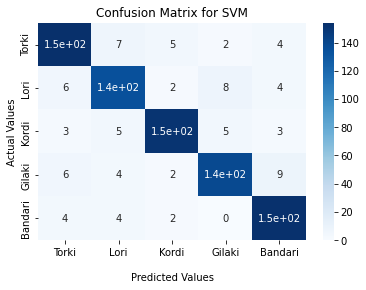
\includegraphics[width=0.75\linewidth]{images/svm_cm_augment.png}
	\caption{ماتریس کانفیوژن دست آمده برای الگوریتم \lr{SVM}}
	\label{fig:svm_cm_augment}
\end{figure}


\begin{figure}[h!]
	\centering
	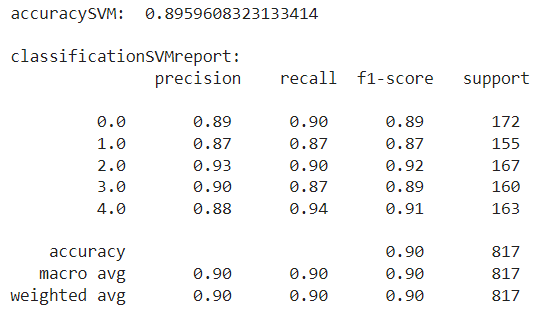
\includegraphics[width=0.9\linewidth]{images/svm_classification_results_augment.PNG}
	\caption{نتایج حاصل به دست آمده برای الگوریتم \lr{SVM}}
	\label{fig:svm_classification_results_augment}
\end{figure}
\newpage
\subsubsection{\lr{: MLP}}
ساختار شبکه در اینجا دو لایه با 128 و 32 نورون به همراه توابع فعالساز \lr{ReLu} در نظر گرفته شد.
نتایج این طبقه بند در ادامه آورده شده است.

\begin{figure}[h!]
	\centering
	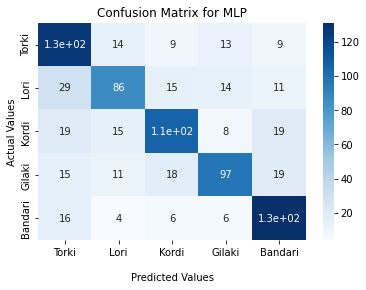
\includegraphics[width=0.75\linewidth]{images/mlp_cm_augment.png}
	\caption{ماتریس کانفیوژن دست آمده برای الگوریتم \lr{MLP}}
	\label{fig:mlp_cm_augment}
\end{figure}

\begin{figure}[h!]
	\centering
	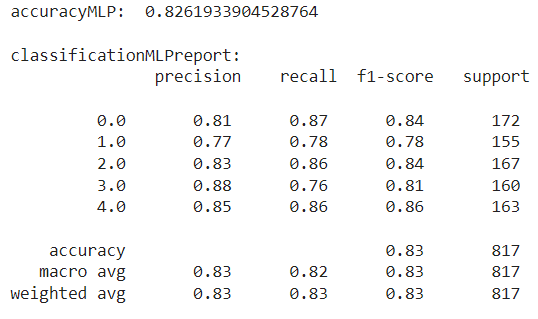
\includegraphics[width=0.9\linewidth]{images/mlp_classification_results_augment.PNG}
	\caption{نتایج حاصل به دست آمده برای الگوریتم \lr{MLP}}
	\label{fig:mlp_classification_results_augment}
\end{figure}
\newpage
\subsubsection{\lr{: KNN}}
نتایج الگوریتم \lr{KNN} با در نظر گرفتن \lr{k=1} در ادامه آورده شده است.

\begin{figure}[h!]
	\centering
	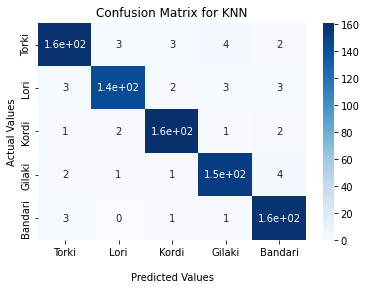
\includegraphics[width=0.75\linewidth]{images/knn_cm_augment.png}
	\caption{ماتریس کانفیوژن دست آمده برای الگوریتم \lr{KNN}}
	\label{fig:knn_cm_augment}
\end{figure}

\begin{figure}[h!]
	\centering
	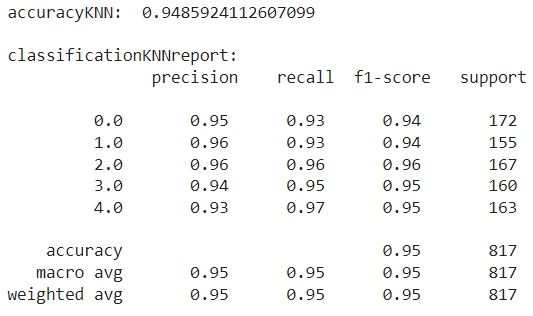
\includegraphics[width=0.9\linewidth]{images/knn_classification_results_augment.PNG}
	\caption{نتایج حاصل به دست آمده برای الگوریتم \lr{KNN}}
	\label{fig:knn_classification_results_augment}
\end{figure}
\newpage
میتوان دید که اضافه کردن داده تاثیر بسیار چشم گیری در عملکرد مدل‌ها دارد، به نحوی که به طور مثال در 
الگوریتم \lr{KNN} توانستیم از دقت 51 درصد به دقت 95 درصد برسیم.
این رشد چشمگیر در سایر الگوریتم‌های طبقه بندی نیز قابل رویت است.

\subsection{\lr{: clustering}}
\subsubsection{\lr{: K Means}}
با همان پارامترهای تنظیم شده برای داده‌های ساده الگوریتم \lr{K Means} را اجرا می‌کنیم نتایج مطابق شکل \ref{fig:kmeans2} می‌باشند.

\begin{figure}[h!]
    \centering
    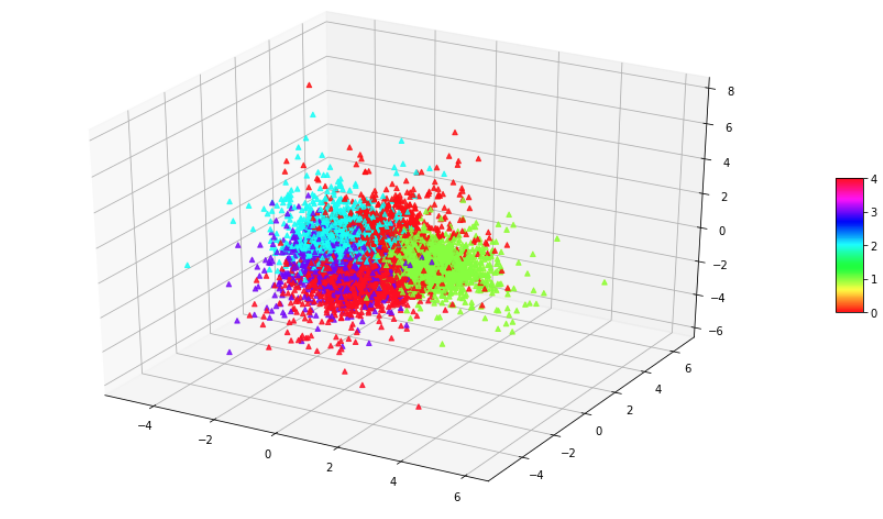
\includegraphics[width=0.65\linewidth]{images/kmeans2.png}
    \caption{نتیجه خوشه بندی با روش \lr{K Means}}
    \label{fig:kmeans2}
\end{figure}

\subsubsection{\lr{: Hierarchical}}
در این قسمت نیز با معیارهای اندازه گیری خوشه \lr{ward}، \lr{complete linkage} و \lr{Average Linkage} الگوریتم طبقه بندی \lr{bottom-up} را اجرا می‌کنیم. و نتایج به شرح زیر می‌باشند.

\begin{figure}[h]
    \centering
    \subfigure[خوشه‌های به دست آمده]{
    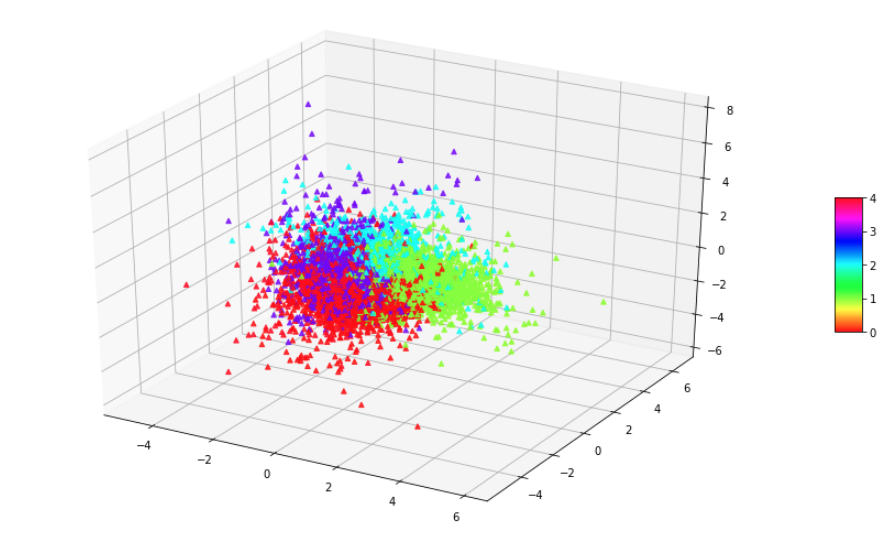
\includegraphics[width=.45\textwidth]{images/ward2.png}
    }
    \subfigure[\lr{Dendogram}]{
    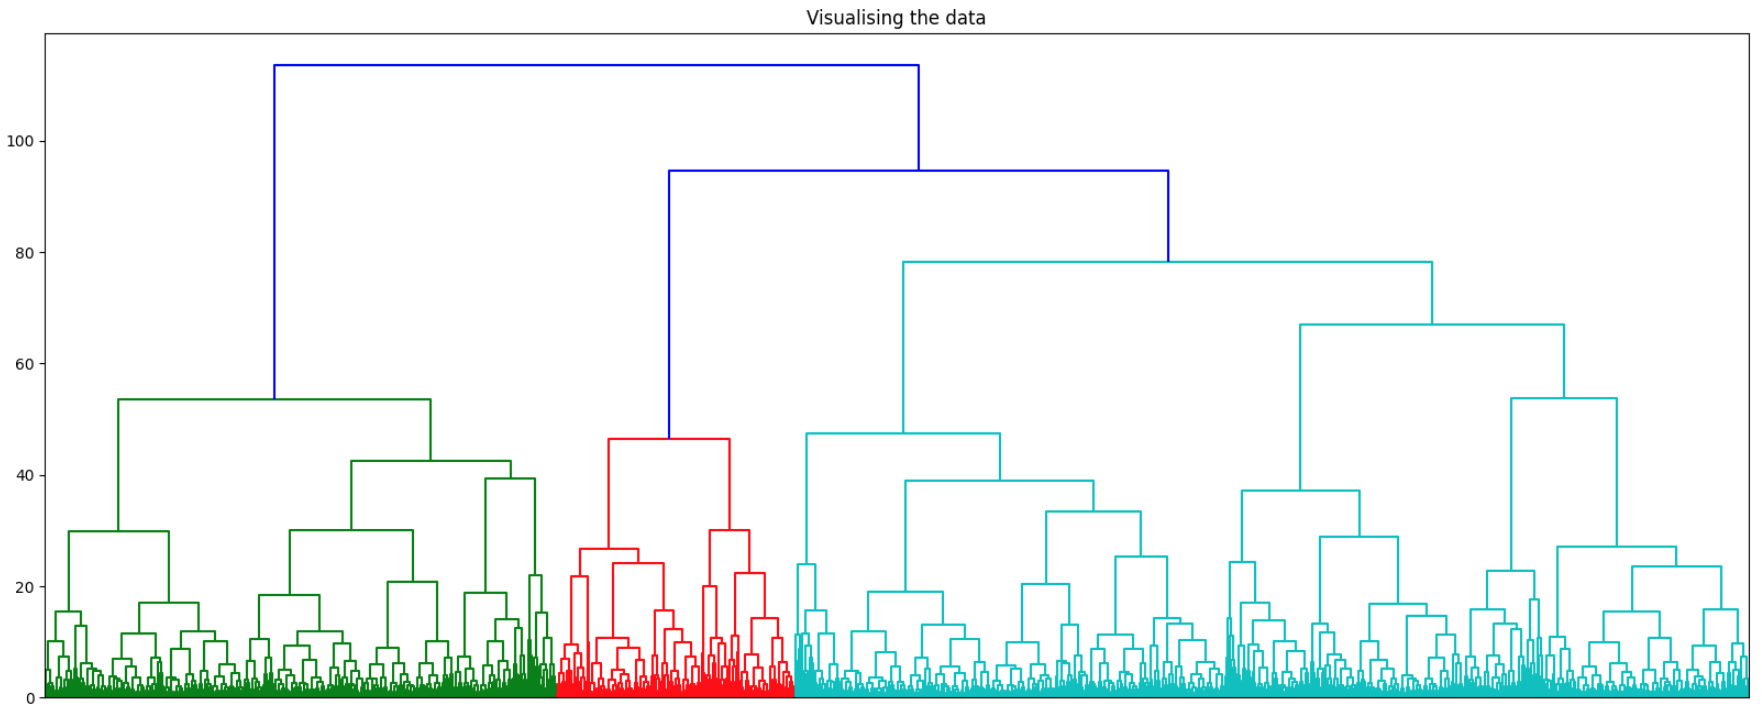
\includegraphics[width=.45\textwidth]{images/ward_dendo2.png}
    }
    \caption{نتیجه خوشه بندی با معیار \lr{ward}}
    \label{fig:ward2}
\end{figure}

\subsubsection{\lr{: DBSCAN}}
این الگوریتم نیز مجددا اجرا شده، اما به همان دلایلی که الگوریتم‌های خوشه بندی عملکرد خوبی در این پروژه نداشتند در این قسمت نیز دقتشان به حد قابل قبولی نرسید.

\begin{figure}[h!]
    \centering
    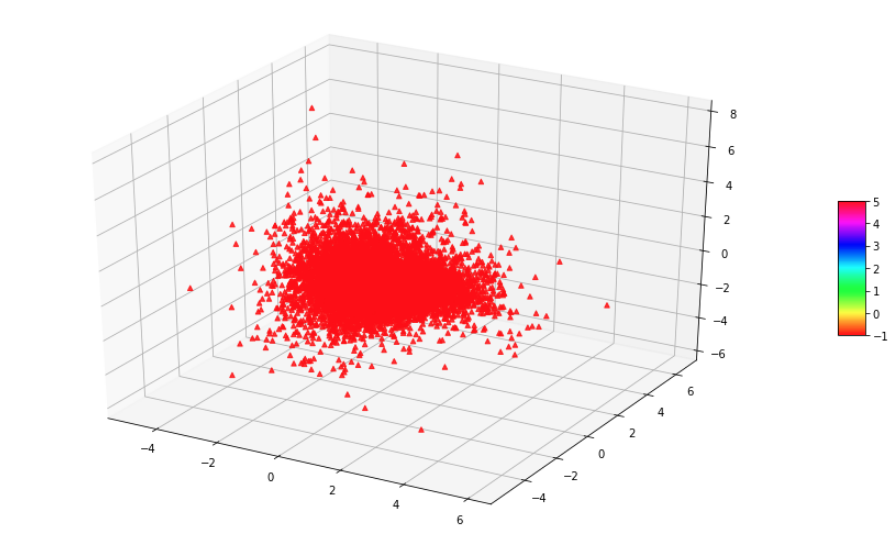
\includegraphics[width=0.65\linewidth]{images/dbscan2.png}
    \caption{نتیجه خوشه بندی با روش \lr{DBSCAN}}
    \label{fig:dbscan2}
\end{figure}
\newpage
\begin{table}[]
	\begin{tabular}{|c|c|c|c|c|c|}
	\hline
	\lr{DBSCAN} & \begin{tabular}[c]{@{}c@{}}\lr{Hierarchical}\\  (\lr{Ward})\end{tabular} & \begin{tabular}[c]{@{}c@{}}\lr{Hierarchical}\\  (\lr{Average})\end{tabular} & \begin{tabular}[c]{@{}c@{}}\lr{Hierarchical} \\ (\lr{Complete})\end{tabular} & \lr{K-Means} & \lr{Measure}    \\ \hline
	\lr{-0.44} & \lr{0.132}                                                          & \lr{0.502}                                                             & \lr{0.128}                                                              & \lr{0.207}   & \lr{Silhouette} \\ \hline
	\lr{0.177}  & \lr{0.167}                                                          & \lr{0.104}                                                             & \lr{0.131}                                                              & \lr{0.228}   & \lr{Purity}     \\ \hline
	\end{tabular}
	\end{table}

\newpage

\section{نمایش داده ها در ابعاد پایین تر} 
برای اینکه بتوانیم کیفیت فیچرهای استخراج شده و کارایی آن‌ها برای انجام این پروژه داده‌ها را در فضای کاهش بعد یافته نمایش می‌دهیم تا به طور کیفی تفکیک پذیری آن‌ها با توجه به فیچرهای استخراج شده مشخص شود.
\\
برای این کار دو الگوریتم \lr{LDA} و \lr{PCA} را در طول ترم یاد گرفیتم. از آن جا که \lr{LDA} با توجه به لیبل داده‌ها جهت‌های بهینه برای تصویر سازی را می‌یابد انتظار داریم داده‌ها پس از انتقال بر روی بردارهای به دست آمده از \lr{LDA} تفکیک پذیری بیشتری نسبت به داده‌ها پس از انتقال با استفاده از \lr{PCA} داشته باشند.
\\ 
پس از کاهش بعد داده‌ها با استفاده از \lr{PCA} بر روی سه کامپوننت اول نتایج زیر حاصل شد که به شکل سه بعدی قابل نشان دادن هستند.

\begin{figure}[h!]
    \centering
    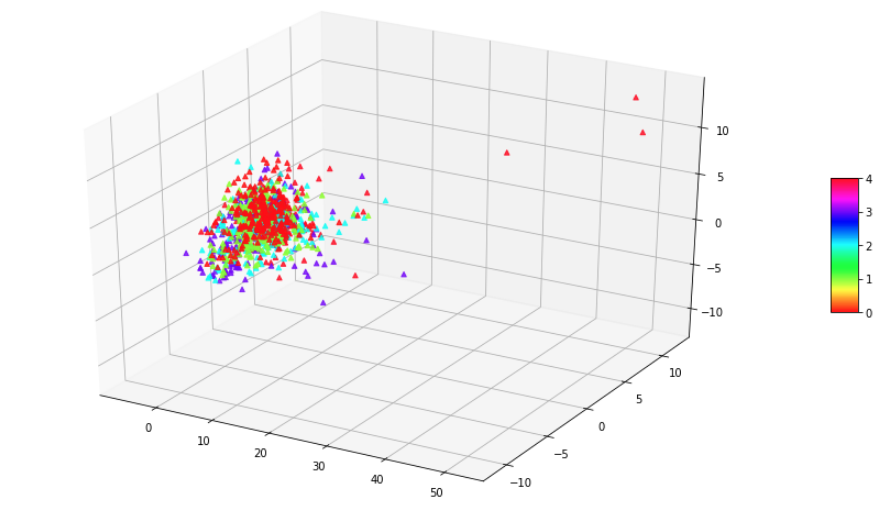
\includegraphics[width=0.5\linewidth]{images/PCA1.png}
    \caption{داده‌های آموزش پس از کاهش بعد با \lr{PCA}}
    \label{fig:pca_vis}
\end{figure}

پس از کاهش بعد داده‌ها با استفاده از \lr{LDA} بر روی سه بردار ویژه اول نتایج زیر حاصل شد که به شکل سه بعدی قابل نشان دادن هستند.

\begin{figure}[h!]
    \centering
    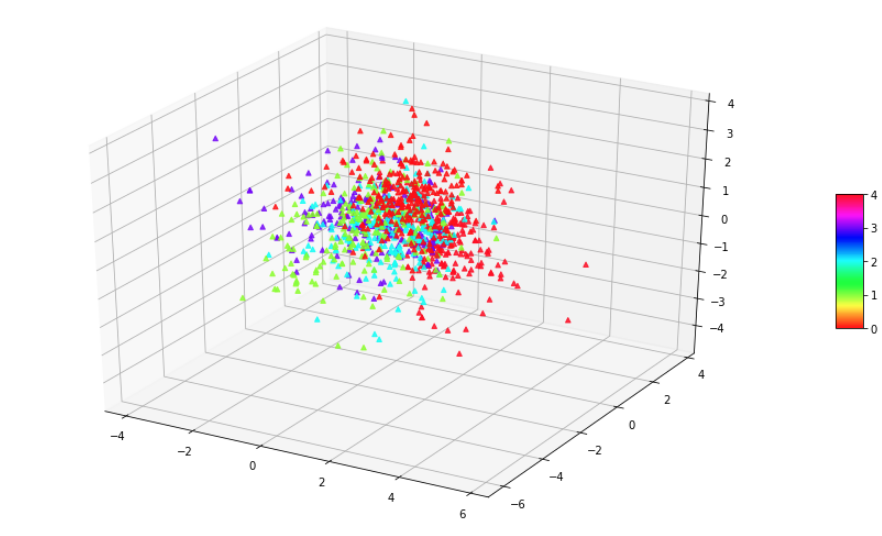
\includegraphics[width=0.5\linewidth]{images/LDA1.png}
    \caption{داده‌های کاهش بعد یافته با استفاده از \lr{LDA}}
    \label{fig:lda_viz}
\end{figure}
        

